% Integration: paste after Section 2; merge bibliography entries into the main bibliography.
% Required packages are listed in ../report.tex. Figure paths are relative to this folder.
\section{Methodology}
\label{sec:methodology}
This study compares five supervised classifiers for Fashion-MNIST: a linear
classifier, a multilayer perceptron (MLP), a convolutional neural network (CNN),
a row-sequence long short-term memory network (LSTM), and a patch-based
Transformer. The comparison examines how different representations and learned
operations classify the same image information under a common data and training
protocol. These are configurations of established model families; the study
does not introduce a new architecture. Model capacity varies, so the experiment
compares complete configurations rather than isolating architecture at a fixed
parameter budget.

\subsection{Overall System Architecture}
\label{sec:meth_system}
The system separates parameter fitting, checkpoint selection, and final
evaluation into distinct stages. A seed-42 stratified partition divides the
60,000 official training images into 54,000 training and 6,000 validation
images. The official 10,000-image test partition retains its supplied examples
and labels. Each class contributes 5,400 training, 600 validation, and 1,000 test
examples. The partition and preprocessing are shared across all five runs;
Figure~\ref{fig:meth_pipeline} shows their information flow.

\begin{figure}[H]\centering
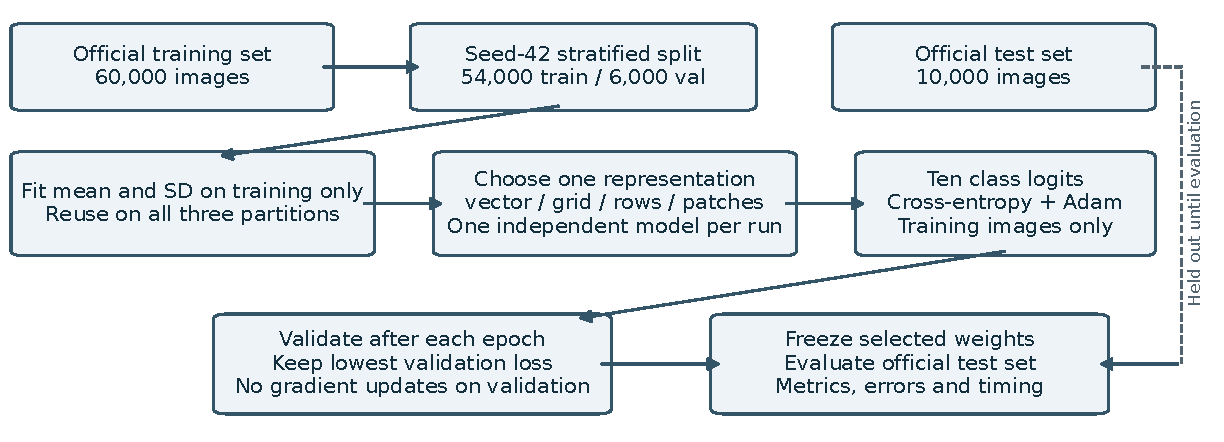
\includegraphics[width=\linewidth]{figures/methodology_pipeline.pdf}
\caption{Shared fitting, selection, and evaluation procedure. Training pixels
fit the normalization, training labels drive Adam updates, and validation loss
selects weights. The test branch evaluates the selected model.}
\label{fig:meth_pipeline}\end{figure}

Each raw grayscale image is converted to a single-channel \texttt{float32}
tensor, scaled by $1/255$, and standardized using the training-only mean
$\mu=0.286209$ and population standard deviation $\sigma=0.353160$ (rounded).
The loader reuses the full-precision cached constants for validation and test
images. Section~2.4 details this transformation; the present section starts
from the resulting standardized image $Z_i\in\mathbb{R}^{1\times28\times28}$.
No augmentation, resizing, sample filtering, or handcrafted features are used.

The representation utility arranges the same 784 standardized values for the
chosen model, as summarized in Table~\ref{tab:meth_inputs}. Here $B$ denotes the
batch size. The target tensor has shape $(B,)$ and contains integer class
indices $y_i\in\{0,\ldots,9\}$ in the dataset's supplied order. Every model
returns ten raw scores, called logits, of shape $(B,10)$. A single model is
trained per run; the five branches do not exchange features or form an ensemble.

\begin{table}[H]\centering
\caption{Input interfaces after common standardization. Sequence order is
spatial within one image.}\label{tab:meth_inputs}
\begin{tabularx}{\linewidth}{l l X}\toprule
Model & Batch shape & Interpretation\\\midrule
Linear / MLP & $(B,784)$ & Pixels flattened row by row.\\
CNN & $(B,1,28,28)$ & Original single-channel spatial grid.\\
LSTM & $(B,28,28)$ & Top-to-bottom rows; 28 left-to-right features per row.\\
Transformer & $(B,49,16)$ & Raster-ordered $4\times4$ patches; row-major pixels within each patch.\\
\bottomrule\end{tabularx}\end{table}

\clearpage
\subsection{Baseline Approach}
\label{sec:meth_baselines}
The linear classifier provides a reference with no learned hidden
representation. It maps the flattened vector $v_i\in\mathbb{R}^{784}$ directly
to ten logits through a fully connected layer with a bias. Its trainable
parameter count is $784\times10+10=7{,}850$. The model can assign different
weights to individual pixel positions, but it cannot learn nonlinear
interactions among them. This makes it a useful starting point for assessing
the effect of learned nonlinear features.

The MLP adds two hidden transformations while retaining the same vector input.
The first layer maps 784 values to 256 features, followed by a rectified linear
unit (ReLU) and dropout with probability 0.2. The second layer maps 256 features
to 128, again followed by ReLU and dropout 0.2. A final $128\to10$ linear layer
produces logits. Its parameter count is
$(784\times256+256)+(256\times128+128)+(128\times10+10)=235{,}146$.
The hidden layers allow nonlinear combinations of pixels, while their dense
connectivity imposes no local spatial weight sharing. Dropout acts during
training and is disabled for validation and test inference.

\subsection{Proposed Models / Algorithms}
\label{sec:meth_models}
The three additional configurations examine local filtering, sequential
aggregation, and attention over image regions. The term ``proposed models''
identifies the models selected for this assignment; it does not imply that
CNNs, LSTMs, or Transformers originate in this work. All models are initialized
and trained from scratch, without pretrained feature extractors.
Figure~\ref{fig:meth_architectures} summarizes their forward paths.

\subsubsection{CNN: Learning Local Spatial Features}
The CNN retains the two-dimensional image grid to learn local patterns through
shared filters, following the convolutional modeling principle of
LeCun et al.~\cite{meth_lecun}. Table~\ref{tab:meth_cnn} gives the exact
forward path. Both convolutions use $3\times3$ kernels, stride 1, padding 1,
and a bias; ReLU follows each convolution. Both max-pooling layers use
$2\times2$ windows with stride 2. The resulting $64\times7\times7$ tensor is
flattened and mapped to 128 features before the output head.

\begin{table}[H]\centering
\caption{CNN operations and output dimensions. The batch axis is retained at
every stage.}\label{tab:meth_cnn}
\begin{tabularx}{\linewidth}{X l}\toprule
Operation & Output shape\\\midrule
Standardized input & $(B,1,28,28)$\\
Convolution $1\to32$, $3\times3$, padding 1; ReLU & $(B,32,28,28)$\\
Max pooling $2\times2$, stride 2 & $(B,32,14,14)$\\
Convolution $32\to64$, $3\times3$, padding 1; ReLU & $(B,64,14,14)$\\
Max pooling $2\times2$, stride 2 & $(B,64,7,7)$\\
Flatten & $(B,3136)$\\
Linear $3136\to128$; ReLU; dropout 0.2 & $(B,128)$\\
Linear $128\to10$ & $(B,10)$\\\bottomrule
\end{tabularx}\end{table}

The CNN has 421,642 trainable parameters: 320 in the first convolution,
18,496 in the second, 401,536 in the hidden dense layer, and 1,290 in the
output layer. Shared convolutional filters provide a local spatial inductive
bias, while pooling reduces spatial resolution and computational demand in
later layers. Pooling also discards precise position information. These
mechanisms motivate the configuration; their effect on classification must
be assessed from the later results.

\clearpage
\subsubsection{LSTM: Reading an Image as an Ordered Row Sequence}
The LSTM processes each image as 28 spatial steps, using one complete row per
step. Removing the single channel axis gives $S_i\in\mathbb{R}^{28\times28}$,
where $S_{i,t,j}=Z_{i,0,t,j}$ for zero-based row and column indices
$t,j\in\{0,\ldots,27\}$. Rows are read from top to bottom, and their features
remain in left-to-right order. The sequence describes a static image rather
than observations over time. No transpose, padding, or truncated sequence is
introduced.

A single unidirectional \texttt{nn.LSTM} layer uses input size 28, hidden
size 128, and \texttt{batch\_first=True}. The hidden and cell states are
initialized to zero independently on each forward call; no state is carried
between images or batches. Processing all rows yields outputs of shape
$(B,28,128)$ and final hidden and cell tensors of shape $(1,B,128)$.
Only the final hidden state is passed through dropout 0.2 and a $128\to10$
linear classifier. There is no inter-layer recurrent dropout because the
network contains one recurrent layer. The LSTM has 82,186 parameters:
$4(128)(28+128+2)=80{,}896$ in the recurrent module, including PyTorch's two
bias vectors, and 1,290 in the classifier.

The recurrent state summarizes the rows encountered so far, providing a
mechanism for combining information across vertical positions. LSTM gating
follows an established recurrent design~\cite{meth_lstm}; the equations below
use the forget-gate form implemented by PyTorch~\cite{meth_torch_lstm}.
Using the final hidden state creates a compact readout, but its sequential
computation and sensitivity to row order are relevant trade-offs.

\subsubsection{Transformer: Attention Across Ordered Image Patches}
The Transformer represents each image as a $7\times7$ grid of nonoverlapping
$4\times4$ patches, producing 49 vectors of length 16. Both patches and their
internal pixels follow row-major order, as defined in Section~2.4. A learned
linear projection maps each patch from 16 to 64 features. A trainable position
embedding of shape $(1,49,64)$ is added before dropout 0.2, allowing tokens
with similar content at different image locations to remain distinguishable.

Two independently initialized encoder blocks preserve the token dimension
$(B,49,64)$. Each block uses four attention heads with 16 features per head,
a $64\to128\to64$ feed-forward network with GELU activation, dropout 0.2,
and pre-normalization residual connections. Internally the code transposes
tokens to $(49,B,64)$ for the encoder layers and transposes them back
afterward. All patches are present, so neither a padding mask nor a causal
mask is supplied. A final layer normalization acts on each token before mean
pooling over the 49 positions, dropout 0.2, and a $64\to10$ classifier.

This configuration uses patch-based visual input~\cite{meth_vit} and
self-attention~\cite{meth_attention}, with no class token or pretrained
weights. Its 71,946 parameters comprise 1,088 in the patch projection, 3,136
in learned positions, 33,472 in each encoder block, 128 in the final layer
normalization, and 650 in the output head. Attention permits interaction
between every pair of image regions within a block; this does not by itself
establish an advantage under a short training budget.

\begin{figure}[H]\centering
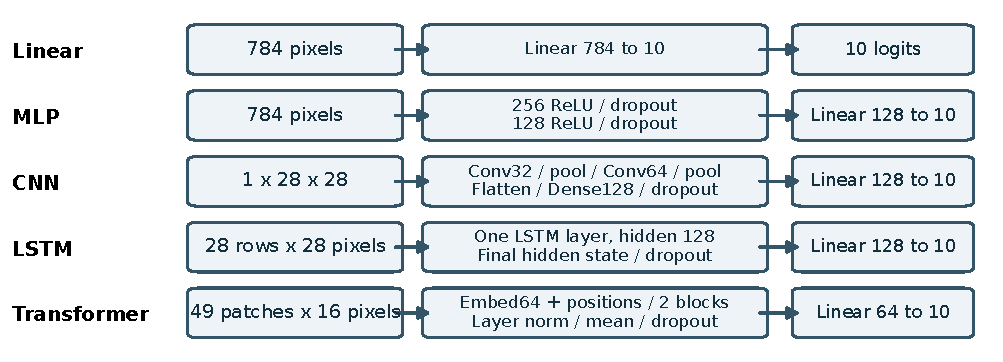
\includegraphics[width=\linewidth]{figures/model_architectures.pdf}
\caption{Implemented forward paths. All five models produce ten logits;
dropout denotes probability 0.2. The Transformer blocks retain 49 tokens.}
\label{fig:meth_architectures}\end{figure}

\clearpage
\subsection{Mathematical Formulation}
\label{sec:meth_math}
\subsubsection{Class Scores and the Learning Objective}
For image $i$, let $\mathcal{R}_m$ denote the input rearrangement for model
$m$ and let $f_{\theta_m}$ be its learned mapping. Classification uses
\begin{equation}
 a_i=f_{\theta_m}(\mathcal{R}_m(Z_i))\in\mathbb{R}^{10},\qquad
 p_{i,k}=\frac{\exp(a_{i,k})}{\sum_{j=0}^{9}\exp(a_{i,j})},\qquad
 \hat y_i=\mathop{\mathrm{arg\,max}}_{k\in\{0,\ldots,9\}}a_{i,k}.
 \label{eq:meth_prediction}
\end{equation}
Here $a_i$ contains raw logits, $p_{i,k}$ is the softmax probability assigned
to class $k$, $\hat y_i$ is the predicted label, and $\theta_m$ contains
the model's trainable parameters. Softmax is used for reported confidence;
the loss receives logits directly for a numerically stable computation.
The maximum probability is not treated as calibrated certainty.

Training minimizes mean cross-entropy over a minibatch $\mathcal{B}$:
\begin{equation}
 \mathcal{L}_{\mathcal{B}}(\theta_m)=
 \frac{1}{|\mathcal{B}|}\sum_{i\in\mathcal{B}}
 \left[-a_{i,y_i}+\log\!\left(\sum_{k=0}^{9}\exp(a_{i,k})\right)\right].
 \label{eq:meth_loss}
\end{equation}
The symbol $|\mathcal{B}|$ is the number of images in the current minibatch
and $y_i$ is its ground-truth class. No class weights, label smoothing, or
additional penalty terms are supplied. Epoch loss averages over images,
weighting each batch by its actual size so that the smaller final batch does
not receive disproportionate weight.

\subsubsection{Dense and Convolutional Transformations}
The linear baseline computes $a_i=Wv_i+b$, with
$W\in\mathbb{R}^{10\times784}$ and $b\in\mathbb{R}^{10}$. For the MLP,
let $\rho(u)=\max(0,u)$ elementwise and let $D$ denote dropout 0.2 during
training and the identity map during evaluation. Its computation is
\begin{equation}
 h_1=D(\rho(W_1v_i+b_1)),\qquad
 h_2=D(\rho(W_2h_1+b_2)),\qquad a_i=W_3h_2+b_3.
 \label{eq:meth_mlp}
\end{equation}
The hidden vectors have dimensions 256 and 128, respectively.
$W_1,W_2,W_3$ have shapes $256\times784$, $128\times256$, and
$10\times128$, with biases matching their output dimensions.
Training dropout independently zeros an activation with probability 0.2 and
rescales retained values by $1/0.8$.

The CNN uses the cross-correlation operation conventionally called
convolution in deep-learning libraries. For an input map $A$ with $C$
channels, an output channel $o$, and padded spatial indices $r,c$, it computes
\begin{equation}
 H_{o,r,c}=\rho\!\left(b_o+
 \sum_{q=0}^{C-1}\sum_{u=0}^{2}\sum_{v=0}^{2}
 K_{o,q,u,v}A_{q,r+u-1,c+v-1}\right),\qquad
 M_{o,r,c}=\max_{u,v\in\{0,1\}} H_{o,2r+u,2c+v}.
 \label{eq:meth_conv}
\end{equation}
$K$ and $b_o$ are the learned kernel and bias, $H$ is the post-ReLU feature
map, and $M$ is the pooled map. Values of $A$ outside its spatial extent are
zero. For the first block, $A=Z_i$ and $C=1$; for the second, $A$ is the
first pooled map and $C=32$. Flattening the second pooled map produces 3,136
features for the dense readout in Table~\ref{tab:meth_cnn}.

\subsubsection{LSTM State Update and Readout}
At recurrent step $t\in\{1,\ldots,28\}$, let $x_t=S_{i,t-1,:}$ be the
28-feature row vector. PyTorch's LSTM computes
\begin{equation}
 \begin{aligned}
 \iota_t&=\operatorname{sigmoid}(W_{xi}x_t+W_{hi}h_{t-1}+b_i),&
 f_t&=\operatorname{sigmoid}(W_{xf}x_t+W_{hf}h_{t-1}+b_f),\\
 g_t&=\tanh(W_{xg}x_t+W_{hg}h_{t-1}+b_g),&
 o_t&=\operatorname{sigmoid}(W_{xo}x_t+W_{ho}h_{t-1}+b_o),\\
 c_t&=f_t\odot c_{t-1}+\iota_t\odot g_t,&
 h_t&=o_t\odot\tanh(c_t).
 \end{aligned}\label{eq:meth_lstm}
\end{equation}
The input, forget, and output gates $\iota_t,f_t,o_t$, candidate $g_t$,
cell state $c_t$, and hidden state $h_t$ are all 128-dimensional.
Each $W_{x\cdot}$ has shape $128\times28$, each $W_{h\cdot}$ has shape
$128\times128$, and each $b_{\cdot}$ combines the corresponding input and
recurrent bias vectors. The operator $\odot$ denotes elementwise
multiplication. With $h_0=c_0=0$, the classifier uses
$a_i=W_{\mathrm{out}}D(h_{28})+b_{\mathrm{out}}$, where
$W_{\mathrm{out}}\in\mathbb{R}^{10\times128}$.

\clearpage
\subsubsection{Patch Embedding, Self-Attention, and Pooling}
For one image, let $P\in\mathbb{R}^{49\times16}$ contain its ordered patch
vectors as rows. Patch projection and positional encoding initialize the
token matrix:
\begin{equation}
 T^{(0)}=D(PW_E+\mathbf{1}_{49}b_E^{\mathsf T}+E),\qquad
 T^{(0)}\in\mathbb{R}^{49\times64}.
 \label{eq:meth_embed}
\end{equation}
Here $W_E\in\mathbb{R}^{16\times64}$ is the embedding matrix,
$b_E\in\mathbb{R}^{64}$ its bias, $\mathbf{1}_{49}$ a column of 49 ones,
and $E\in\mathbb{R}^{49\times64}$ the learned position matrix shared
across images. Each row of $E$ identifies one location in the patch grid.

Each encoder block first normalizes its input tokens and computes attention
over all 49 positions. For a normalized token matrix
$U\in\mathbb{R}^{49\times64}$ and head $h\in\{1,2,3,4\}$, the operation is
\begin{equation}
 Q_h=UW_h^Q+\mathbf{1}_{49}(b_h^Q)^{\mathsf T},\quad
 K_h=UW_h^K+\mathbf{1}_{49}(b_h^K)^{\mathsf T},\quad
 V_h=UW_h^V+\mathbf{1}_{49}(b_h^V)^{\mathsf T},
 \label{eq:meth_qkv}
\end{equation}
\begin{equation}
 A_h=D_A\!\left[\operatorname{softmax}_{\mathrm{row}}
       \left(\frac{Q_hK_h^{\mathsf T}}{\sqrt{16}}\right)\right]V_h,
 \qquad
 \operatorname{MHA}(U)=\operatorname{Concat}(A_1,A_2,A_3,A_4)W_O
                   +\mathbf{1}_{49}b_O^{\mathsf T}.
 \label{eq:meth_attention}
\end{equation}
Each projection $W_h^{Q},W_h^{K},W_h^{V}$ has shape $64\times16$,
with a 16-dimensional bias. Thus $Q_h,K_h,V_h,A_h$ have shape
$49\times16$, and the attention weights have shape $49\times49$.
Row-wise softmax normalizes the key positions for each query position.
$D_A$ denotes dropout 0.2 on attention weights during training.
Concatenation joins heads along the feature axis; the output projection
$W_O\in\mathbb{R}^{64\times64}$ and $b_O\in\mathbb{R}^{64}$ restore
64 features per token.

The pre-normalized residual path of block $\ell\in\{1,2\}$ is
\begin{equation}
 \begin{aligned}
 R^{(\ell)}&=T^{(\ell-1)}+
       D\!\left(\operatorname{MHA}_{\ell}
          (\operatorname{LN}_{\ell,1}(T^{(\ell-1)}))\right),\\
 T^{(\ell)}&=R^{(\ell)}+
       D\!\left(\operatorname{FFN}_{\ell}
          (\operatorname{LN}_{\ell,2}(R^{(\ell)}))\right),\\
 \operatorname{FFN}_{\ell}(U)&=
       D\!\left(\operatorname{GELU}(UW_{\ell,1}
                    +\mathbf{1}_{49}b_{\ell,1}^{\mathsf T})\right)
                    W_{\ell,2}+\mathbf{1}_{49}b_{\ell,2}^{\mathsf T}.
 \end{aligned}\label{eq:meth_block}
\end{equation}
$R^{(\ell)}$ is the intermediate residual matrix and $T^{(\ell)}$ the block
output. Each $\operatorname{LN}$ is a learned layer normalization over the
64 features of a token, with $\epsilon=10^{-5}$. The feed-forward weights
$W_{\ell,1}\in\mathbb{R}^{64\times128}$ and
$W_{\ell,2}\in\mathbb{R}^{128\times64}$ act independently at every token;
their biases have dimensions 128 and 64. GELU denotes the Gaussian error
linear unit. Every occurrence of $D$ uses an independent dropout mask during
training. This sequence matches the implemented
\texttt{norm\_first=True} encoder~\cite{meth_torch_encoder}.

After the second block, a separate layer normalization precedes mean pooling:
\begin{equation}
 r_i=\frac{1}{49}\sum_{j=1}^{49}
       [\operatorname{LN}_{\mathrm{final}}(T^{(2)})]_{j,:}^{\mathsf T},\qquad
 a_i=W_C D(r_i)+b_C.
 \label{eq:meth_pool}
\end{equation}
Here the column vector $r_i\in\mathbb{R}^{64}$ averages normalized token features,
$W_C\in\mathbb{R}^{10\times64}$ is the classifier weight, and
$b_C\in\mathbb{R}^{10}$ its bias. All 49 patches contribute to the pooled readout.
Layer normalization is applied before averaging, which is distinct from
normalizing only the final pooled vector.

\clearpage
\subsection{Training Strategy}
\label{sec:meth_training}
The primary comparison fixes the partition, input transformation, optimizer,
batch size, epoch budget, and checkpoint policy. Table~\ref{tab:meth_training}
lists the shared settings. This protocol controls several sources of variation
while allowing the architectures and their parameter counts to differ.
Ten epochs provide the same number of passes over training data, rather than
the same runtime or proof of convergence for every architecture.

\begin{table}[H]\centering
\caption{Verified common training protocol. Architecture-specific dropout
locations are described in Sections~3.2--3.3.}\label{tab:meth_training}
\begin{tabularx}{\linewidth}{l X}\toprule
Setting & Value or policy\\\midrule
Partition & Seed-42 stratified 54,000 / 6,000 split; official test retained\\
Normalization & Training-only global mean and population SD; reused unchanged\\
Random control & Python, NumPy, and PyTorch seeds 42; seeded training shuffle\\
Optimizer & Adam; learning rate $10^{-3}$, $\beta_1=0.9$, $\beta_2=0.999$, $\epsilon=10^{-8}$\\
Budget and batches & 10 complete epochs; batch size 128; final partial batch retained\\
Loss & Mean multiclass cross-entropy; no class weighting or label smoothing\\
Regularization & Dropout 0.2 in MLP, CNN, LSTM, and Transformer; none in Linear\\
Augmentation & Disabled for training, validation, and test\\
Other optimization & Weight decay 0; no scheduler, gradient clipping, or early stopping\\
Data loading & Training shuffled; validation/test ordered; zero worker processes\\
Numerical execution & Float32 model/input computation; no mixed-precision training\\
Checkpoint & Lowest validation cross-entropy; first epoch retained on an exact tie\\
\bottomrule\end{tabularx}\end{table}

Each training minibatch first clears gradients, then computes logits and the
mean loss in Equation~\ref{eq:meth_loss}. Backpropagation produces gradients,
and Adam updates the trainable parameters using its running first- and
second-moment estimates~\cite{meth_adam}. The process visits all 54,000
training images once per epoch: 421 full batches and one final batch of 112
images. This yields 422 updates per epoch and 4,220 updates per model.
Validation follows every epoch with the model in evaluation mode and gradient
recording disabled. Validation loss, accuracy, and macro-F1 are recorded, but
only validation loss controls checkpoint replacement.

Let $\theta_m^{(e)}$ denote the weights after epoch $e$ and
$\mathcal{L}_{\mathrm{val}}$ the mean loss across all validation images.
The selected checkpoint is
\begin{equation}
 e_m^*=\min\!\left\{e:\mathcal{L}_{\mathrm{val}}(\theta_m^{(e)})
     =\min_{s\in\{1,\ldots,10\}}
       \mathcal{L}_{\mathrm{val}}(\theta_m^{(s)})\right\},\qquad
 \theta_m^*=\theta_m^{(e_m^*)}.
 \label{eq:meth_selection}
\end{equation}
The outer minimum resolves a tie in favor of the earlier epoch. All ten
epochs run even if an earlier checkpoint is selected. The saved checkpoint
contains model weights, model identity, selected epoch, configuration,
normalization constants, input mode, and source/split fingerprints. It does
not contain optimizer state for exact training resumption. The cached indices
and split fingerprint identify the partition; they are not inferred from
test performance.

Random seeds are reset before model initialization. Built-in PyTorch layer
initialization is retained, except that Transformer position embeddings use
a truncated normal with standard deviation 0.02. The two encoder blocks are
constructed separately. cuDNN benchmarking is disabled and deterministic
cuDNN behavior is requested; the implementation does not enable a global
deterministic-algorithms guarantee. A fixed seed therefore supports
reproducibility without implying bitwise equality across devices or versions.

The saved baseline Linear and MLP runs record MPS training, whereas CNN,
LSTM, and Transformer record CUDA training on the GTX 1660 SUPER. These are
historical runs with a shared statistical protocol, not a matched hardware
timing study. The separate shared-CUDA configuration is a future rerun
protocol, not evidence of five completed CUDA training runs. The test set has
already been evaluated in the project; later repetitions cannot be described
as first access to previously unseen test data.

\clearpage
\subsection{Evaluation Metrics}
\label{sec:meth_metrics}
Evaluation reloads the validation-selected checkpoint, verifies its source
and split fingerprints and normalization constants against the data loader,
and computes predictions without parameter updates. The official test set
is used for reporting generalization under the stated protocol. No test score
is used by the implemented checkpoint-selection rule. Prediction records
retain each example's test index, true label, predicted label, confidence,
and correctness, allowing aggregate metrics to be checked against individual
outcomes.

\subsubsection{Predictive Performance and Class-Specific Errors}
For an evaluation partition of $N$ images, accuracy is
\begin{equation}
 \operatorname{Accuracy}=\frac{1}{N}\sum_{i=1}^{N}
       \mathbb{I}(\hat y_i=y_i).
 \label{eq:meth_accuracy}
\end{equation}
$\mathbb{I}(\cdot)$ equals one for a true condition and zero otherwise.
The denominator is 6,000 for validation and 10,000 for official-test reporting.
Values may be reported as fractions or percentages, with units stated.

The confusion matrix $C\in\mathbb{N}_0^{10\times10}$ counts true classes
in rows and predicted classes in columns: $C_{a,b}$ is the number of images
with label $a$ predicted as $b$. For class $k$, define
$\mathrm{TP}_k=C_{k,k}$,
$\mathrm{FP}_k=\sum_{a\ne k}C_{a,k}$, and
$\mathrm{FN}_k=\sum_{b\ne k}C_{k,b}$. Precision, recall, and F1 are
\begin{equation}
 \mathrm{Precision}_k=\frac{\mathrm{TP}_k}{\mathrm{TP}_k+\mathrm{FP}_k},\quad
 \mathrm{Recall}_k=\frac{\mathrm{TP}_k}{\mathrm{TP}_k+\mathrm{FN}_k},\quad
 \mathrm{F1}_k=\frac{2\mathrm{TP}_k}
 {2\mathrm{TP}_k+\mathrm{FP}_k+\mathrm{FN}_k},\qquad
 \mathrm{MacroF1}=\frac{1}{10}\sum_{k=0}^{9}\mathrm{F1}_k.
 \label{eq:meth_f1}
\end{equation}
An undefined per-class score is assigned zero, matching the class-report
convention. Class support is $\sum_bC_{k,b}$, which is 1,000 for each
official-test class. Macro-F1 gives each category equal weight. It complements
accuracy by exposing uneven class performance; it is the mean of individual
class F1 scores, not the F1 computed from macro-averaged precision and recall.
Test loss is the summed cross-entropy divided by 10,000. Confusion matrices,
class scores, and seed-fixed correct/incorrect image grids support later
error analysis without placing results in this methodology section.

\subsubsection{Model Size and Timing Boundaries}
Model size is measured by the number of trainable scalar parameters, including
biases, learned positions, and layer-normalization parameters. Counts are
recomputed from instantiated models and checked against saved summaries.
Parameter count describes storage and capacity, but does not determine runtime
because architectures perform different operations.

Forward timing uses a fixed device-resident batch of 128 images in inference
mode. Ten forward calls warm up execution; the next 100 calls are timed with
device synchronization before and after the interval. If their total duration
is $T_{100}$ seconds, the reported batch time is $1000T_{100}/100$
milliseconds and amortized time per image is that value divided by 128.
This excludes loading and host-to-device transfers and measures batched
forward cost rather than single-request response time. A separate complete
test-pass timer includes data loading, transfers, forward computation, loss,
predictions, and confidence extraction; it excludes plotting and artifact
writing after the pass. The current evaluator reports one aggregate timing
interval, not a distribution of independent timing repetitions.

The training timer covers the ten-epoch training/validation loop, epoch
logging, and saves of improved checkpoints, with device synchronization at
its boundaries. It excludes initial data preparation, model/optimizer
construction, and post-loop re-evaluation and artifact generation. Historical
MPS and CUDA training durations must be labeled by device and must not form
a matched cross-model speed ranking. Peak allocated or reserved GPU memory
is not measured by the existing trainer/evaluator, so no peak-memory result
is asserted here. Such a comparison requires explicitly instrumented runs
under the same device and measurement scope.
